\documentclass{VUMIFPSkursinis}
\usepackage{algorithmicx}
\usepackage{algorithm}
\usepackage{algpseudocode}
\usepackage{amsfonts}
\usepackage{amsmath}
\usepackage{bm}
\usepackage{caption}
\usepackage{color}
\usepackage{float}
\usepackage{graphicx}
\usepackage{listings}
\usepackage{subfig}
\usepackage{wrapfig}
\usepackage{pdflscape} %Keep it to pdflscape or I can't rotate my diagram (K.S.)
\usepackage{longtable}
\usepackage[table]{xcolor}
\usepackage{multirow}
\usepackage[usestackEOL]{stackengine}
\usepackage{longtable}
\usepackage{subfig}
\usepackage{wrapfig}


\usepackage{enumitem}
%PAKEISTA, tarpai tarp sąrašo elementų
\setitemize{noitemsep,topsep=0pt,parsep=0pt,partopsep=0pt}
\setenumerate{noitemsep,topsep=0pt,parsep=0pt,partopsep=0pt}

% Titulinio aprašas
\university{Vilniaus universitetas}
\faculty{Matematikos ir informatikos fakultetas}
\department{Programų sistemų katedra}
\papertype{Programų sistemų inžinerijos I laboratorinis darbas Nr. 2}
\title{Kavinės staliuko rezervavimo aplikacija}
\titleineng{Cafe table rezervation app}
\status{2 kurso 5 grupės studentai}
\author{Paulius Grigaliūnas}
\secondauthor{Karolis Staskevičius}
\thirdauthor{Modestas Dulevičius}
\fourthauthor{Albert Jurkoit}
\fifthauthor{Šarūnas Kazimieras Buteikis}
     

% \secondauthor{Vardonis Pavardonis}   % Pridėti antrą autorių
\supervisor{dr. Vytautas Valaitis}
\date{Vilnius – \the\year}

% Nustatymai
% \setmainfont{Palemonas}   % Pakeisti teksto šriftą į Palemonas (turi būti įdiegtas sistemoje)

\begin{document}
% PAKEISTA	
\maketitle
\cleardoublepage\pagenumbering{arabic}
\setcounter{page}{2}


%ANOTACIJA

\sectionnonum{ANOTACIJA}
\noindent
Šiame dokumente detaliai išdėstomi kavinės rezervavimo sistemos reikalavimai. Remiantis dalykinės srities analize pateikiama vartotojo interfeiso, funkcinių ir nefunkcinių programų sistemos reikalavimų specifikacija, kuria siekiama užtikrinti standartartizuotos bei funkcionalios sistemos sukūrimą.\\\\




%TURINYS(TOC)
\tableofcontents

%ĮVADAS
\sectionnonum{Įvadas}
\noindent
Kavinės rezervavimo aplikacija kuriama siekiant išplėsti kavinių staliukų rezervavimą nuotoliniu būdu Lietuvoje, suteikti galimybę klientams paprastai ir patogiai užsisakyti staliuką bet kuriuo paros metu bei padėti savininkams susilaukti daugiau lankytojų. 
\newline
Dokumente pateikiamos programos savybės ir tam tikri ribojimai jos kūrimui, kuriais turi pasižymėti sistema. Pateikiami vartotojo sąsajos funkciniai bei nefunkciniai reikalavimai, sekų diagramos, iliustruojančios, kaip sistema turi veikti.\\\\
{\bfseries Programų sistemos pavadinimas}\\\\
Pilnas programų sistemos pavadinimas – kavinės rezervavimo „Covfefe“ aplikacija. Trumpas sistemos pavadinimas – "Covfefe“.\\\\
{\bfseries Dalykinė sritis}\\\\
Kavinės ir jų rezervacija.\\\\
\noindent
{\bfseries Probleminė sritis}\\\\
Programelė̇ suteikia galimybę užsirezervuoti staliuką pasirinktoje kavinėje internetu. "Covfefe" sprendžia problemą, kad šiandieninėje rinkoje žmogus neturi galimybės vienoje aplikacijoje užsirezvuoti staliuką skirtingose kavinėse.\\\\
{\bfseries Naudotojai}\\\\
Klientas. Reikalingos bazinės naudojimosi kompiuteriu bei internetu žinios (kompiuterinis raštingumas).\\\
Kavinės savininkas. Reikalingas kompiuterinis raštingumas, gebėjimas tinkamai užpildyti formos laukus.\\\\
{\bfseries Darbo pagrindas}\\\\
Dokumentas parengtas kaip programų sistemų inžinerijos kurso antrasis laboratorinis darbas.
\newline

%FUNKCINIAI REIKALAVIMAI

\section{Vartotojo sąsaja}

\subsection{Formuluojamos užduotys}
\subsubsection{Kliento užduotys}
\begin{center}
	\begin{table}[H]
	\caption{Kliento užduotys}
	\begin{tabular}{|p{2cm}|p{2,5cm}|p{9,6cm}|}
	\hline
	    \rowcolor{lightgray}
		\multicolumn{3}{|c|}{Kliento užduotys}\\
		
	\hline
		\multicolumn{1}{|c|}{{\bfseries Kodas}}&
		\multicolumn{1}{|c|}{{\bfseries Užduotis}}&
		\multicolumn{1}{|c|}{{\bfseries Formulavimo būdas}}\\		
	\hline
		\multicolumn{1}{|c|}{VS 1.1.1}& 	
		\multicolumn{1}{|c|}{Autentifikavimo užduotys}&
		{
			\begin{enumerate}
				\item Registruotis sistemoje
				(privalomi duomenys:vardas, pavardė, el. paštas, telefono numeris, slaptažodis).
				\item Prisijungti prie sistemos (privalomi duomenys: el. paštas, slaptažodis).
				\item “Premium” prisijungimas (aktyvuojamas klientui, kuris nupirko tam tikrą paslaugą) leidžiantis prisijungti prie sistemos vienu mygtuko paspaudimu.
			\end{enumerate}}\\
	
	\hline
		\multicolumn{1}{|c|}{VS 1.1.2}&  	
		\multicolumn{1}{|c|}{Pagalbinės užduotys}&
		{
			\begin{enumerate}
				\item Peržiūrėti visas sistemoje registruotas kavinės, informaciją apie jas.
				\item Ieškoti kavinę pagal vardą.
				\item Ieškoti kavinę pagal vietą.
				\item Peržiūrėti pasirinktos kavinės detaliąją informaciją (Vardas, adresas, staliukų skaičius, darbo grafikas).
				\item Rezervuoti staliuką pasirinktoje kavinėje.
			\end{enumerate}}\\
	
	\hline 	 	
	\end{tabular}

	\label{table:1}
	\end{table}

\end{center}

\subsubsection{Kavinės savininko užduotys}
\begin{center}
	\begin{table}[H]
	\begin{tabular}{|p{2cm}|p{2,5cm}|p{9,6cm}|}
	\hline
	    \rowcolor{lightgray}
		\multicolumn{3}{|c|}{Kavinės savininko užduotys}\\
		
	\hline
		\multicolumn{1}{|c|}{{\bfseries Kodas}}&
		\multicolumn{1}{|c|}{{\bfseries Užduotis}}&
		\multicolumn{1}{|c|}{{\bfseries Formulavimo būdas}}\\		
	\hline
		\multicolumn{1}{|c|}{VS 1.2.1}&  	
		\multicolumn{1}{|c|}{Autentifikavimo užduotys}&
		{
			\begin{enumerate}
				\item Registruotis sistemoje (privalomi duomenys:vardas, pavardė, el. paštas, telefono numeris, slaptažodis).
				\item Prisijungti prie sistemos (privalomi duomenys: el. paštas, slaptažodis).
			\end{enumerate}}\\
	\hline
		\multicolumn{1}{|c|}{VS 1.2.2}&
		\multicolumn{1}{|c|}{Pagalbinės užduotys}&
		{
			\begin{enumerate}
				\item Pridėti kavinę (privalomi duomenys: kavinės vardas, adresas, staliukų skaičius, darbo grafikas. Papildomi: kavinės telefono numeris).
				\item Peržiūrėti sistemoje registruotų kavinių sąrašą.
				\item Atnaujinti informaciją apie savo registruotą kavinę.
			\end{enumerate}}\\
	
	\hline 	 	
	\end{tabular}
	\caption{Kavinės savininko užduotys}
	\label{table:2}
	\end{table}

\end{center}

\subsection{Užduočių formulavimo kalbos reikalavimai}
\begin{center}

	\begin{longtable}{|p{2cm}|p{4,1cm}|p{9,6cm}|}
	\caption{Užduočių formulavimo kalbos reikalavimai}
	\endfirsthead
	\endhead
	\hline
	    \rowcolor{lightgray}
		\multicolumn{3}{|c|}{Užduočių formulavimo kalbos reikalavimai}\\
		
	\hline
		\multicolumn{1}{|c|}{{\bfseries Kodas}}&
		\multicolumn{1}{|c|}{{\bfseries Užduotis}}&
		\multicolumn{1}{|c|}{{\bfseries Formulavimo būdas}}\\		
	\hline
		\multicolumn{1}{|c|}{VS 2.1}& 	
		{Registruotis}&
		\multicolumn{1}{|p{8,6cm}|}{
			\begin{enumerate}
				\item Duomenų įvedimo laukeliai.
				\item Registracijos mygtukas.
			\end{enumerate}}\\
	
	\hline
		\multicolumn{1}{|c|}{VS 2.2}& 	
		{Prisijungti}&
		\multicolumn{1}{|p{8,6cm}|}{
			\begin{enumerate}
				\item Piktrograma. 
				\item Duomenų įvedimo laukeliai.
				\item Prisijungimo  mygtukas.
			\end{enumerate}}\\
	
	\hline
		\multicolumn{1}{|c|}{VS 2.3}& 	
		{Premium prisijungimas}&
		\multicolumn{1}{|p{8,6cm}|}{
			\begin{enumerate}
				\item Premium prisijungimo mygtukas.
			\end{enumerate}}\\
	
	\hline
		\multicolumn{1}{|c|}{VS 2.4}& 	
		{Kavinės pridėjimas}&
		\multicolumn{1}{|p{8,6cm}|}{
			\begin{enumerate}
				\item Duomenų įvedimo laukeliai.
				\item Pridėjimo mygtukas.
			\end{enumerate}}\\
	
	\hline 	
		\multicolumn{1}{|c|}{VS 2.5}&
		\multicolumn{1}{|c|}{Išeiti}&
		\multicolumn{1}{|p{8,6cm}|}{
			\begin{enumerate}
				\item Išėjimo mygtukas.
			\end{enumerate}}\\
	
	\hline	
		\multicolumn{1}{|c|}{VS 2.6}&
		{Kavinės paieška}&
		\multicolumn{1}{|p{10,2cm}|}{
			\begin{enumerate}
				\item Lentelė su sistemoje registruotomis kavinėmis.
				\item Kavinės rezervacijos mygtukas.
				\item Paieškos duomenų įvedimo laukelis.
				\item Paieškos pagal vardą mygtukas.
				\item Paieškos pagal vietą mygtukas.
				\item Parodyti daugiau informacijos mygtukas.
			\end{enumerate}}\\
	
	\hline 	
		\multicolumn{1}{|c|}{VS 2.7}&
		{Kavinės rezervacija}&
		\multicolumn{1}{|p{10,2cm}|}{
			\begin{enumerate}
				\item Datos (metai, mėnuo, diena) nustatymo laukelis
				\item Laiko (valandos, minutės) nustatymo laukelis.
				\item Lango uždarymo mygtukas.
				\item Rezervacijos mygtukas.
			\end{enumerate}}\\
	
	\hline
		\multicolumn{1}{|c|}{VS 2.8}& 	
		{Kavinės informacijos atnaujinimas}&
		\multicolumn{1}{|p{8,6cm}|}{
			\begin{enumerate}
				\item Duomenų įvedimo laukeliai.
				\item Patvirtinimo mygtukas.
			\end{enumerate}}\\
	
	\hline
	
	\label{table:3}	
	\end{longtable}

\end{center}

\pagebreak

\begin{landscape}
\subsection{Užduočių formulavimo būdo(protokolo) reikalavimai}
	\begin {figure}[H]
		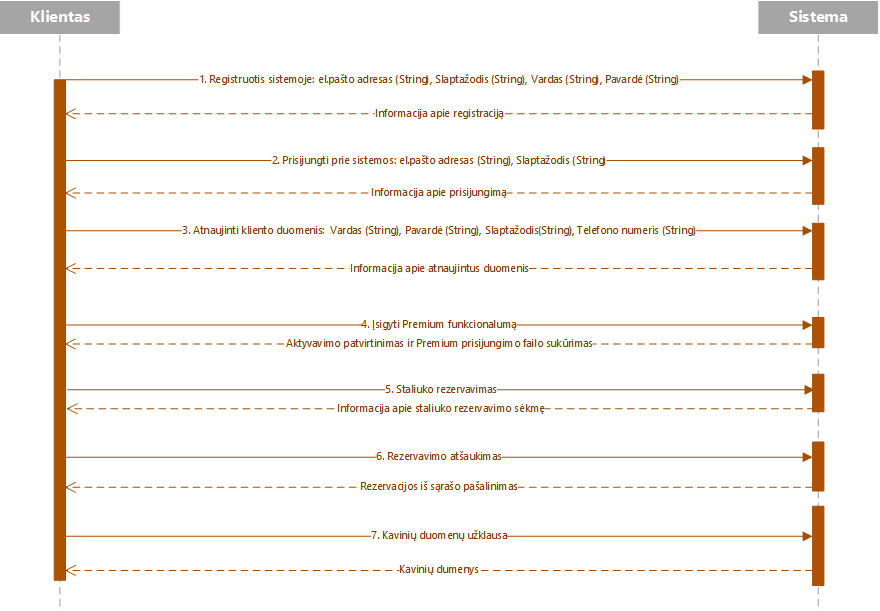
\includegraphics[width=1.2\textwidth,height=1.3\textheight,keepaspectratio]{img/b}
		\caption{Kliento registracija sistemoje}
		\label{fig:b}
	\end{figure}
\end{landscape}

\begin{landscape}
	\begin {figure}[H]
		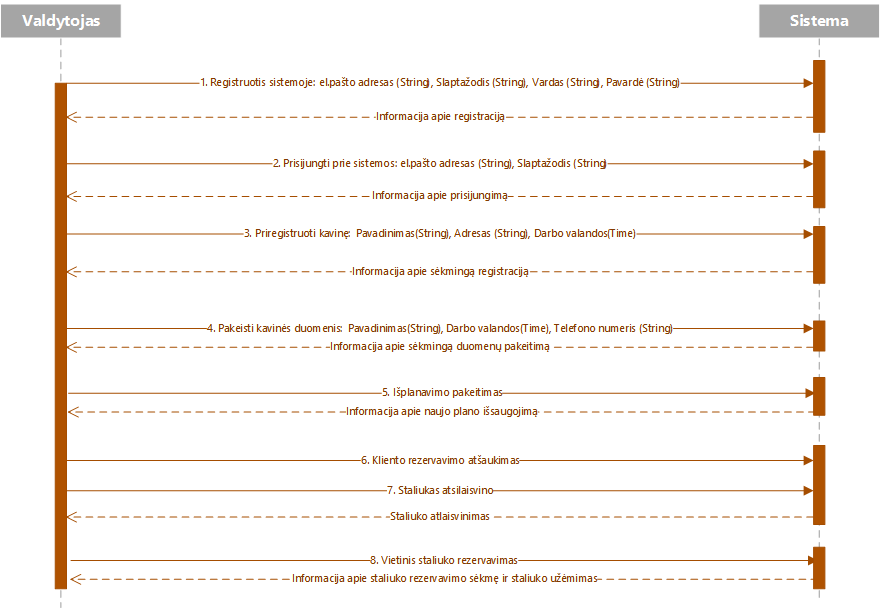
\includegraphics[width=1.3\textwidth,height=1.4\textheight,keepaspectratio]{img/c}
		\caption{Kavinės savininko registracija sistemjoe}
		\label{fig:c}
	\end{figure}
\end{landscape}


\subsection{Interfeiso darnos ir standartizavimo reikalavimai}
\begin{center}
	\begin{table}[H]
	\caption{Interfeiso darnos ir standartizavimo reikalavimai}
	\begin{tabular}{|p{2cm}|p{14cm}|p{2cm}|}
	\hline
	    \rowcolor{lightgray}
	    \multicolumn{3}{|c|}{Interfeiso darnos ir standartizavimo reikalavimai}\\
	\hline
		\multicolumn{1}{|c|}{{\bfseries Kodas}}&
		\multicolumn{1}{|c|}{ {\bfseries Užduotis}}&
		\multicolumn{1}{|c|}{{\bfseries Svarba}}\\		
	\hline
		\multicolumn{1}{|c|}{VS 3.1}&
		\multicolumn{1}{|p{12,9cm}|}{Pagrindinis meniu visuomet pasiekiamas paspaudus ant programėlės logotipo esančio kairiajame viršutiniame kampe.}& 
		\multicolumn{1}{|p{1.5cm}|}{PAGEIDAUTINA}\\
	\hline
		\multicolumn{1}{|c|}{VS 3.2}&
		\multicolumn{1}{|p{12cm}|}{Languose dominuoja „Royal Jewels“ spalvų paletė.}& 
		\multicolumn{1}{|p{1.5cm}|}{PAGEIDAUTINA}\\
	\hline
		\multicolumn{1}{|c|}{VS 3.3}&
		\multicolumn{1}{|p{12cm}|}{Tekstui naudojami ‚Times New Roman“ šriftas}& 
		\multicolumn{1}{|p{1.5cm}|}{PAGEIDAUTINA}\\
	\hline  	 	
	
	\end{tabular}
	
	\label{table:4}
	\end{table}

\end{center}

\subsection{Pranešimų formulavimo reikalavimai}
\begin{center}
	\begin{table}[H]
	\caption{Pranešimų formulavimo reikalavimai}
	\begin{tabular}{|p{2cm}|p{11cm}|p{2cm}|}
	\hline
	    \rowcolor{lightgray}
	    \multicolumn{3}{|c|}{Pranešimų formulavimo reikalavimai}\\
	\hline
		\multicolumn{1}{|c|}{{\bfseries Kodas}}&
		\multicolumn{1}{|c|}{ {\bfseries Užduotis}}&
		\multicolumn{1}{|c|}{{\bfseries Svarba}}\\		
	\hline
		\multicolumn{1}{|c|}{VS 4.1}&
		\multicolumn{1}{|p{12,6cm}|}{Pranešimų tekstas turi būti parašytas laikantis gramatikos ir skyrybos taisyklių.}& 
		\multicolumn{1}{|c|}{BŪTINA}\\
	\hline
		\multicolumn{1}{|c|}{VS 4.2}&
		\multicolumn{1}{|p{12,5cm}|}{Pranešime vartojami tik interfeiso naudotojams žinomi terminai, vengiama žargonų ir svetimybių, tačiau leistina vartoti dalykinės srities metaforas.}& 
		\multicolumn{1}{|c|}{BŪTINA}\\
	\hline
		\multicolumn{1}{|c|}{VS 4.3}&
		\multicolumn{1}{|p{12,5cm}|}{Informacinio tipo pranešimai aprašys domenų įvedimo kriterijus.}& 
		\multicolumn{1}{|c|}{BŪTINA}\\
	\hline
		\multicolumn{1}{|c|}{VS 4.4}&
		\multicolumn{1}{|p{12,5cm}|}{Pranešimų langai įspės apie blogai įvestus duomenis, pavyzdžiui, per trumpą įvestą slaptažodį arba jau užregistruotą el. paštą.}& 
		\multicolumn{1}{|c|}{BŪTINA}\\
	\hline
		\multicolumn{1}{|c|}{VS 4.5}&
		\multicolumn{1}{|p{12,5cm}|}{Pranešimas turi pateikti informaciją apie sėkmingai atliktą veiksmą arba informuoti apie klaidą.}& 
		\multicolumn{1}{|c|}{BŪTINA}\\
	\hline
		\multicolumn{1}{|c|}{VS 4.6}&
		\multicolumn{1}{|p{12,5cm}|}{Pranešimo tekstas turi būti suprantamas vienareikšmiškai.}& 
		\multicolumn{1}{|c|}{BŪTINA}\\
	\hline
		\multicolumn{1}{|c|}{VS 4.7}&
		\multicolumn{1}{|p{12,5cm}|}{Pranešimas apie klaidą turi būti detalus.}& 
		\multicolumn{1}{|p{1.5cm}|}{PAGEIDAUTINA}\\
	\hline
		\multicolumn{1}{|c|}{VS 4.8}&
		\multicolumn{1}{|p{12,5cm}|}{Informacinis pranešimas turi būti žalios arba mėlynos spalvos, o klaidos pranešimas - raudonos.}& 
		\multicolumn{1}{|p{1.5cm}|}{PAGEIDAUTINA}\\
	\hline
		\multicolumn{1}{|c|}{VS 4.9}&
		\multicolumn{1}{|p{12,5cm}|}{Pradinis pranešimo langas negali užimti daugiau nei 50\% ekrano pločio ir aukščio.}& 
		\multicolumn{1}{|p{1.5cm}|}{PAGEIDAUTINA}\\
	\hline
		\multicolumn{1}{|c|}{VS 4.10}&
		\multicolumn{1}{|p{12,5cm}|}{Pranešimo teksto ilgis negali viršyti 100 simbolių limito.}& 
		\multicolumn{1}{|p{1.5cm}|}{PAGEIDAUTINA}\\
	\hline
		\multicolumn{1}{|c|}{VS 4.11}&
		\multicolumn{1}{|p{12,5cm}|}{Pranešimas turi turėti antraštę.}& 
		\multicolumn{1}{|p{1.5cm}|}{PAGEIDAUTINA}\\
	\hline
		\multicolumn{1}{|c|}{VS 4.12}&
		\multicolumn{1}{|p{12,5cm}|}{Turi būti galimybė išjungti pranešimo langą.}& 
		\multicolumn{1}{|c|}{BŪTINA}\\
	\hline	 	
	
	\end{tabular}
	
	\label{table:5}
	\end{table}

\end{center}

\pagebreak

\subsection{Interfeiso individualizavimo reikalavimai}

\begin{center}
	\begin{table}[H]
	\caption{Interfeiso individualizavimo reikalavimai}
	\begin{tabular}{|p{2cm}|p{13cm}|p{2cm}|}
	\hline
	    \rowcolor{lightgray}
	    \multicolumn{3}{|c|}{Interfeiso individualizavimo reikalavimai}\\
	\hline
		\multicolumn{1}{|c|}{ {\bfseries Kodas}}&
		\multicolumn{1}{|c|}{ {\bfseries Užduotis}}&
		\multicolumn{1}{|c|}{{\bfseries Svarba}}\\		
	\hline
		\multicolumn{1}{|c|}{VS 5.1}&
		\multicolumn{1}{|p{12,9cm}|}{Ekrano temos pasirinkimas (minimalūs dizaino pakeitimai: spalva, šriftas)}& 
		\multicolumn{1}{|p{1.5cm}|}{PAGEIDAUTINA}\\
	\hline
		\multicolumn{1}{|c|}{VS 5.1}&
		\multicolumn{1}{|p{12,9cm}|}{Kalbos pasirinkimas.}& 
		\multicolumn{1}{|p{1.5cm}|}{PAGEIDAUTINA}\\
	\hline
	
	\end{tabular}
	
	\label{table:6}	
	\end{table}
\end{center}

\section{Funkciniai reikalavimai}
%PRADEDAME RASYTI LENTELES WOHOO

Šiame skyriuje bus nurodomi aplikacijos funkciniai reikalavimai ir jų įgyvendinimo svarba.

\subsection{Aplikacijos langai}

 %APLIKACIJOS LANGAI
\begin{center}
	\begin{table}[H]
	\caption{Aplikacijos langų funkciniai reikalavimai.}
	\begin{tabular}{|p{2cm}|p{12,5cm}|p{3,5cm}|}
	\hline
	    \rowcolor{lightgray}
		\multicolumn{3}{|c|}{Aplikacijos langai}\\
		
	\hline
		\multicolumn{1}{|c|}{{\bfseries Kodas}}&
		\multicolumn{1}{|c|}{{\bfseries Reikalavimas}}&
		\multicolumn{1}{|c|}{{\bfseries Svarba}}\\

	\hline
		\multicolumn{1}{|c|}{FR 1.1} &
		Iš visų aplikacijos langų galima grįžti į prisijungimo langą &
		\multicolumn{1}{|c|}{BŪTINA}\\
	\hline
		\multicolumn{1}{|c|}{FR 1.2} &
		{Visi langai po prisijungimo turi turėti galimybę parodyti kliento \newline prisijungimo vardą/paštą.}&
		\multicolumn{1}{|c|}{BŪTINA}\\
	\hline
	
		\multicolumn{1}{|c|}{FR 1.3}&
		{Jeigu klientas turi rezervavęs staliuką - iš visų langų, išskyrus \newline prisijungimo, galima patekti į langą rodantį rezervacijos informaciją.}&
		\multicolumn{1}{|c|}{BŪTINA}\\
	\hline
		\multicolumn{1}{|c|}{FR 1.4}&
		{Iš prisijungimo lango galima patekti į registracijos ir meniu langą.}&
		\multicolumn{1}{|c|}{BŪTINA}\\
	\hline
		\multicolumn{1}{|c|}{FR 1.5}&
		{Iš meniu lango galima patekti į:\newline
		\begin{enumerate}
			\item Jei prisijungia kavinės administratorius:
				\begin{enumerate}
					\item “Keisti kavinės informaciją” langą.
					\item “Keisti kavinės išplanavimą” langą.
				\end{enumerate}
			\item Jei prisijungia kavinės darbuotojas:
				\begin{enumerate}
					\item “Lokali rezervacija” langą.
				\end{enumerate}
			\item Jei prisijungia klientas:
				\begin{enumerate}
					\item “Kavinės paieška” langas.
				\end{enumerate}
			\item Visi prisijungę klientai turi galimybę patekti į “Keisti kliento duomenis” langą.
			\item Visi langai turi turėti galimybę grįžti į ankstesnį langą.
		\end{enumerate}
		}&
		\multicolumn{1}{|c|}{BŪTINA}\\		
	\hline
	
	\end{tabular}
	
	\label{table:AplikacijosLangai}
	\end{table}
	
\end{center}

\pagebreak

\subsection{Kliento registracija}
%Vartotojo prisijungimas
\begin{center}

	\begin{table}[H]
	\caption{Kliento registracijos funkciniai reikalavimai}
	\begin{tabular}{|p{2cm}|p{12,5cm}|p{3,5cm}|}
	\hline
	    \rowcolor{lightgray}
		\multicolumn{3}{|c|}{Kliento registracija}\\
		
	\hline
		\multicolumn{1}{|c|}{{\bfseries Kodas}}&
		\multicolumn{1}{|c|}{{\bfseries Reikalavimas}}&
		\multicolumn{1}{|c|}{{\bfseries Svarba}}\\

	\hline
	\multicolumn{1}{|c|}{FR 2.1}&
	{Klientas, norintis registruotis prie aplikacijos, turi nurodyti:
		\begin{itemize}
			\item Vardą.
			\item Pavardę.
			\item Slaptažodį.
			\item Telefono numerį (neprivaloma).
			\item Elektroninį paštą.
		\end{itemize}}&		
	\multicolumn{1}{|c|}{BŪTINA}\\
	\hline
	
		\multicolumn{1}{|c|}{FR 2.2}&
		{Informuoti klientą apie sėkmingą registraciją}&
		\multicolumn{1}{|c|}{BŪTINA}\\	
	\hline
		\multicolumn{1}{|c|}{FR 2.3}&
		{Kliento duomenys išsaugomi duomenų bazėje}&
		\multicolumn{1}{|c|}{BŪTINA}\\	
	\hline	
		\multicolumn{1}{|c|}{FR 2.4}&
		{Tam, kad įvestas kliento el. pašto adresas būtų tinkamos formos, jis turi būti sudarytas iš abonento vardo, „@“ simbolio bei domeno adreso.}&
		\multicolumn{1}{|c|}{BŪTINA}\\	
	\hline
		\multicolumn{1}{|c|}{FR 2.5}&
		{Slaptažodis privalo būti sudarytas bent iš 8 simbolių, turi bent vieną skaitmenį.
}&
		\multicolumn{1}{|c|}{BŪTINA}\\		
	\hline
		\multicolumn{1}{|c|}{FR 2.6}&
		{Duomenų bazėje išsaugomi kliento duomenys turi būti string tipo }&
		\multicolumn{1}{|p{1.5cm}|}{PAGEIDAUTINA}\\		
	\hline
	
	\end{tabular}
	
	\label{table:VartotojoRegistracija}
	\end{table}

\end{center}

\subsection{Kliento prisijungimas}

\begin{center}
	\begin{table}[H]
	\caption{Kliento prisijungimo funkciniai reikalavimai}
	\begin{tabular}{|p{2cm}|p{12,5cm}|p{3,5cm}|}
	\hline
	    \rowcolor{lightgray}
		\multicolumn{3}{|c|}{Kliento prisijungimas}\\
		
	\hline
		\multicolumn{1}{|c|}{{\bfseries Kodas}}&
		\multicolumn{1}{|c|}{{\bfseries Reikalavimas}}&
		\multicolumn{1}{|c|}{{\bfseries Svarba}}\\

	\hline
	
		\multicolumn{1}{|c|}{FR 3.1}&
		{Klientas, norintis prisijungti prie aplikacijos turi nurodyti:
			\begin{itemize}
				\item Elektroninio pašto adresas.
				\item Slaptažodis.
			\end{itemize}
		}&
		\multicolumn{1}{|c|}{BŪTINA}\\	
		
	\hline	
		\multicolumn{1}{|c|}{FR 3.2}&
		{Klientas prijungiamas prie sistemos ir nukreipiamas į meniu langą kartu su papildomais kliento duomenimis.}&
		\multicolumn{1}{|c|}{BŪTINA}\\
		
	\hline	
		\multicolumn{1}{|c|}{FR 3.3}&
		{Jei prisijungimo duomenys neteisingi, klientas informuojamas pranešimu.}&
		\multicolumn{1}{|c|}{BŪTINA}\\		
		
	\hline
		\multicolumn{1}{|c|}{FR 3.4}&
		{Kliento įvesti duomenys (slaptažodis bei el. pašto adresas) turi būti sutikrinti su duomenimis, esančiais duomenų bazėje.}&
		\multicolumn{1}{|c|}{BŪTINA}\\
		
	\hline	
		\multicolumn{1}{|c|}{FR 3.5}&
		{Jei prisijungimo duomenys neteisingi, klientas informuojamas pranešimu.}&
		\multicolumn{1}{|c|}{BŪTINA}\\
	\hline
	
	
	
	\end{tabular}	
	
	\label{table:VartotojoPrisijungimas}		
	\end{table}

\end{center}
\pagebreak

\subsection{Kavinės pasirinkimas}

\begin{center}
	\begin{table}[H]
	\caption{Kavinės pasirinkimo funkciniai reikalavimai}
	\begin{tabular}{|p{2cm}|p{12,5cm}|p{3,5cm}|}
	
	\hline
	    \rowcolor{lightgray}
		\multicolumn{3}{|c|}{Kavinės pasirinkimas}\\
		
	\hline
		\multicolumn{1}{|c|}{{\bfseries Kodas}}&
		\multicolumn{1}{|c|}{{\bfseries Reikalavimas}}&
		\multicolumn{1}{|c|}{{\bfseries Svarba}}\\

	\hline
	
		\multicolumn{1}{|c|}{FR 4.1}&
		{Klientui pateikiamas sąrašas arčiausiai jo esančių kavinių kartu su jų duomenimis (ne visais):
		\begin{itemize}
			\item Pavadinimas.
			\item Adresas.
			\item Reitingas.
		\end{itemize}}&
		\multicolumn{1}{|c|}{BŪTINA}\\	
		
	\hline
	
		\multicolumn{1}{|c|}{FR 4.2}&
		{Klientas gali paspausti ir pasirinkti vieną iš kavinių.}&
		\multicolumn{1}{|c|}{BŪTINA}\\
		
	\hline
	
		\multicolumn{1}{|c|}{FR 4.4}&
		{Klientui pasirinkus kavinę, parodoma visa jos informacija:
		\begin{itemize}
			\item Pavadinimas.
			\item Adresas.
			\item Vietų skaičius.
			\item Laivų vietų skaičius.
			\item Reitingas.
			\item Darbo valandos.
		\end{itemize}}&
		\multicolumn{1}{|c|}{BŪTINA}\\
		
	\hline
	
		\multicolumn{1}{|c|}{FR 4.5}&
		{Klientas, pasirinkęs kavinę (turinčią laisvų vietų), gali užsisakyti staliuką.}&
		\multicolumn{1}{|c|}{BŪTINA}\\
	\hline
	
		\multicolumn{1}{|c|}{FR 4.6}&
		{Jeigu klientas nori užsisakyti staliuką, jis yra nukreipiamas į staliuko užsakymo langą}&
		\multicolumn{1}{|c|}{BŪTINA}\\				
	\hline
	
	\end{tabular}		
	
	\label{table:KavinėsPasirinkimas}
	\end{table}


\end{center}

\pagebreak


\subsection{Staliuko užsakymas}
\begin{center}
	\begin{table}[H]
	\caption{Staliuko užsakymo funkciniai reikalavimai.}
	\begin{tabular}{|p{2cm}|p{12,5cm}|p{3,5cm}|}
	
	\hline
	    \rowcolor{lightgray}
		\multicolumn{3}{|c|}{Staliuko užsakymas}\\
		
	\hline
		\multicolumn{1}{|c|}{{\bfseries Kodas}}&
		\multicolumn{1}{|c|}{{\bfseries Reikalavimas}}&
		\multicolumn{1}{|c|}{{\bfseries Svarba}}\\

	\hline
	
		\multicolumn{1}{|c|}{FR 5.1}&
		{Klientui pateikiamas kavinės išplanavimas su staliukais.}&
		\multicolumn{1}{|c|}{BŪTINA}\\				
	\hline
	
		\multicolumn{1}{|c|}{FR 5.2}&
		{Klientas pasirinkęs vieną iš laisvų staliukų nukreipiamas į langą, kuriame prašo įvesti rezervacijos datą ir laiką.}&
		\multicolumn{1}{|c|}{BŪTINA}\\				
	\hline
	
		\multicolumn{1}{|c|}{FR 5.3}&
		{Jei klientas nėra Premium ir kavinėje likęs tik vienas laisvas staliukas - klientas neturi galimybės jo rezervuoti, gauna pranešimą, kad neturi Premium privilegijų.}&
		\multicolumn{1}{|c|}{BŪTINA}\\				
	\hline
	
		\multicolumn{1}{|c|}{FR 5.4}&
		{Klientas norėdamas rezervuoti vietą restorane privalo nurodyti:
			\begin{itemize}
				\item Rezervavimo datą.
				\item Rezervavimo laiką.
			\end{itemize}}&
			\multicolumn{1}{|c|}{BŪTINA}\\				
	\hline
	
		\multicolumn{1}{|c|}{FR 5.3}&
		{Duomenų bazėje patikrinus ar staliukas vis dar laisvas į ją siunčiamas rezervacijos data ir laikas, kartu su užsisakiusio kliento vardu, paštu ir telefono numeriu (jei yra įvestas)}&
		\multicolumn{1}{|c|}{BŪTINA}\\				
	\hline
	
			
	
	\end{tabular}		
	
	\label{table:StaliukoUžsakymas}
	\end{table}


\end{center}

\pagebreak

\subsection{Rezervacijų peržiūra}
\begin{center}
	\begin{table}[H]
	\caption{Rezervacijos peržiūros funkciniai reikalavimai.}
	\begin{tabular}{|p{2cm}|p{12,5cm}|p{3,5cm}|}
	
	\hline
	    \rowcolor{lightgray}
		\multicolumn{3}{|c|}{Rezervacijų priežiūra}\\
		
	\hline
		\multicolumn{1}{|c|}{{\bfseries Kodas}}&
		\multicolumn{1}{|c|}{{\bfseries Reikalavimas}}&
		\multicolumn{1}{|c|}{{\bfseries Svarba}}\\

	\hline
	
		\multicolumn{1}{|c|}{FR 6.1}&
		{Klientas mato savo rezervacijų sąrašą.}&
		\multicolumn{1}{|c|}{BŪTINA}\\				
	\hline
	
		\multicolumn{1}{|c|}{FR 6.2}&
		{Klientas mato savo rezervacijų sąrašą.}&
		\multicolumn{1}{|c|}{BŪTINA}\\				
	\hline
	
		\multicolumn{1}{|c|}{FR 6.3}&
		{Vykdant rezervacijos atšaukimą į duomenų bazę siunčiama užklausa atlaisvinti staliuką. Rezervacijos įrašas pašalinamas iš kliento rezervacijos sąrašo.}&
		\multicolumn{1}{|c|}{BŪTINA}\\				
	\hline
	
		\multicolumn{1}{|c|}{FR 6.4}&
		{Klientas gali peržiūrėti kavinės rezervaciją. Peržiūrint kavinės informaciją pateikiamas kavinės duomenų langas.}&
		\multicolumn{1}{|c|}{BŪTINA}\\				
	\hline		
	
	\end{tabular}		
	
	\label{tabel:RezervacijosPeržiūra}
	\end{table}


\end{center}



\subsection{Kavinės įvertinimas}
\begin{center}
	\begin{table}[H]
	\caption{Kavinės įvertinimo funkciniai reikalavimai}
	\begin{tabular}{|p{2cm}|p{12,5cm}|p{3,5cm}|}
	
	\hline
	    \rowcolor{lightgray}
		\multicolumn{3}{|c|}{Kavinės įvertinimas}\\
		
	\hline
		\multicolumn{1}{|c|}{{\bfseries Kodas}}&
		\multicolumn{1}{|c|}{{\bfseries Reikalavimas}}&
		\multicolumn{1}{|c|}{{\bfseries Svarba}}\\

	\hline
	
		\multicolumn{1}{|c|}{FR 7.1}&
		{Kavinės valdytojui pažymėjus, kad prieš tai kliento rezervuotas staliukas atsilaisvino, klientas gauna langą, kuriame prašoma įvertinti kavinę.}&
		\multicolumn{1}{|c|}{BŪTINA}\\				
	\hline
	
		\multicolumn{1}{|c|}{FR 7.2}&
		{Klientas gali atsisakyti įvertinti kavinę.}&
		\multicolumn{1}{|c|}{BŪTINA}\\				
	\hline
	
		\multicolumn{1}{|c|}{FR 7.3}&
		{Atsisakius įvertinti kavinę, automatiškai išeinama iš kavinės įvertinimo lango.}&
		\multicolumn{1}{|c|}{BŪTINA}\\				
	\hline
	
		\multicolumn{1}{|c|}{FR 7.4}&
		{Klientas gali įvertinti kavinę nuo 1 iki 5}&
		\multicolumn{1}{|c|}{BŪTINA}\\				
	\hline
	
		\multicolumn{1}{|c|}{FR 7.5}&
		{Įvertinus kavinę, rezultatas yra siunčiamas į duomenų bazę ir kavinės reitingas yra atnaujinamas. Išeinama iš kavinės vertinimo lango.}&
		\multicolumn{1}{|c|}{BŪTINA}\\				
	\hline	
	
	\end{tabular}		
	
	\label{table:KavinėsĮvertinimas}
	\end{table}


\end{center}
\pagebreak

\subsection{Kavinės planavimas}
\begin{center}
	\begin{table}[H]
	\caption{Kavinės planavimo funkciniai reikalavimai}
	\begin{tabular}{|p{2cm}|p{12,5cm}|p{3,5cm}|}
	
	\hline
	    \rowcolor{lightgray}
		\multicolumn{3}{|c|}{Kavinės planavimas}\\
		
	\hline
		\multicolumn{1}{|c|}{{\bfseries Kodas}}&
		\multicolumn{1}{|c|}{{\bfseries Reikalavimas}}&
		\multicolumn{1}{|c|}{{\bfseries Svarba}}\\

	\hline
		\multicolumn{1}{|c|}{FR 8.1}&
		{Kavinės savininkas gali vilkti toliau nurodytas figūras ant pateikto standartinio kavinės plano:
		\begin{itemize}
			\item Įvairūs stalai.
			\item Baro/Kasos stalas.
			\item Kėdės.
			\item Suolai/Sofos.
			\item Iėjimas.
			\item Langai
			\item Dekoratyviniai objektai.
		\end{itemize}}&
		\multicolumn{1}{|c|}{BŪTINA}\\

	\hline
	
		\multicolumn{1}{|c|}{FR 8.2}&
		{Nuvilkus stalą - paprašoma įvesti kiek žmonių gali susėsti prie to stalo.Po to nurodoma pridėti pakankamai kėdžių arba suolų sofų, kol patenkinamas vietų skaičius.}&
		\multicolumn{1}{|c|}{BŪTINA}\\				
	\hline
	
		\multicolumn{1}{|c|}{FR 8.3}&
		{Įvedus kiek žmonių gali sedėti prie stalo nurodoma kiek reikia pridėti kėdžių arba suolų sofų, kol patenkinamas vietų skaičius.}&
		\multicolumn{1}{|c|}{BŪTINA}\\				
	\hline
	
		\multicolumn{1}{|c|}{FR 8.4}&
		{Privaloma pridėti įėjimą.}&
		\multicolumn{1}{|c|}{BŪTINA}\\				
	\hline
	
		\multicolumn{1}{|c|}{FR 8.5}&
		{Privaloma pridėti barą arba kasos stalą.}&
		\multicolumn{1}{|c|}{BŪTINA}\\				
	\hline
	
		\multicolumn{1}{|c|}{FR 8.6}&
		{Kavinės savininkas gali išsaugoti kavinės planą.}&
		\multicolumn{1}{|c|}{BŪTINA}\\				
	\hline
	
		\multicolumn{1}{|c|}{FR 8.7}&
		{Kavinės savininko išsaugotas kavinės planas patalpinamas į duomenų bazę.}&
		\multicolumn{1}{|c|}{BŪTINA}\\				
	\hline
	
	\end{tabular}
	
	\label{table:KavinėsPlanavimas}
	\end{table}
	
	
\end{center}

\pagebreak

\subsection{Kavinės pridėjimas}
\begin{center}
	\begin{table}[H]
	\caption{Kavinės pridėjimas}
	\begin{tabular}{|p{2cm}|p{12,5cm}|p{3,5cm}|}
	
	\hline
	    \rowcolor{lightgray}
		\multicolumn{3}{|c|}{Kavinės pridėjimas}\\
		
	\hline
		\multicolumn{1}{|c|}{{\bfseries Kodas}}&
		\multicolumn{1}{|c|}{{\bfseries Reikalavimas}}&
		\multicolumn{1}{|c|}{{\bfseries Svarba}}\\

	\hline
		\multicolumn{1}{|c|}{FR 9.1}&
		{Jeigu klientas dar nėra sukūręs nei vienos kavinės, pridėdamas naują kavinę, jis automatiškai tampa kavinės savininkas.}&
		\multicolumn{1}{|c|}{BŪTINA}\\	

	\hline
		\multicolumn{1}{|c|}{FR 9.2}&
		{Klientas arba kavinės savininkas gali pridėti naują kavinę, įvesdamas tam tikrus duomenis:
			\begin{itemize}
				\item Privaloma įvesti kavinės pavadinimą.
				\item Privaloma nurodyti kavinės adresą.
				\item Būtina įvesti staliukų skaičių. (bent 1 staliukas).
				\item Privaloma nurodyti kavinės darbo laiką darbo dienomis ir savaitgaliais.
				\item Galima papildomai pridėti savininko telefono numerį.
			\end{itemize}}&
		\multicolumn{1}{|c|}{BŪTINA}\\	

	\hline
		\multicolumn{1}{|c|}{FR 9.3}&
		{Kavinės įvedamų duomenų formatai
			\begin{itemize}
				\item Kavinės pavadinimas (String).
				\item Kavinės adresas (String).
				\item Staliukų skaičius (Int, $>$0).
				\item Darbo dienomis (String).
				\item Šeštadieniais (String).
				\item Sekmadieniais (String).
			\end{itemize}}&
		\multicolumn{1}{|c|}{BŪTINA}\\	

	\hline
		\multicolumn{1}{|c|}{FR 9.4}&
		{Sėkmingai pridėjus kavinę pranešama informacija apie sėkmingai pridėtą kavinę.}&
		\multicolumn{1}{|c|}{BŪTINA}\\	

	\hline
		\multicolumn{1}{|c|}{FR 9.5}&
		{Sėkmingai pridėjus kavinę, jos duomenys išsaugomi duomenų bazėje.}&
		\multicolumn{1}{|c|}{BŪTINA}\\	

	\hline
		\multicolumn{1}{|c|}{FR 9.6}&
		{Kavinės savininkas gali atšaukti kavinės pridėjimą.}&
		\multicolumn{1}{|c|}{BŪTINA}\\	

	\hline
		\multicolumn{1}{|c|}{FR 9.7}&
		{Sėkmingai atšaukus kavinės pridėjimą, automatiškai išeinama iš kavinės pridėjimo lango.}&
		\multicolumn{1}{|c|}{BŪTINA}\\	

	\hline
	
	
	
	\end{tabular}
	
	\label{table:KavinėsPridėjimas}		
	\end{table}

\end{center}


\subsection{Kavinės informacijos keitimas}
\begin{center}
	\begin{table}[H]
	\caption{Kavinės informacijos keitimas}
	\begin{tabular}{|p{2cm}|p{12,5cm}|p{3,5cm}|}
	\hline
	    \rowcolor{lightgray}
		\multicolumn{3}{|c|}{Kavinės informacijos keitimas}\\
		
	\hline
		\multicolumn{1}{|c|}{{\bfseries Kodas}}&
		\multicolumn{1}{|c|}{{\bfseries Reikalavimas}}&
		\multicolumn{1}{|c|}{{\bfseries Svarba}}\\
	\hline 	
		\multicolumn{1}{|c|}{FR 10.1}&
		{Tik kavinės savininkas turi galimybę pakeisti savo pridėtų kavinių informaciją.}&
		\multicolumn{1}{|c|}{BŪTINA}\\
	
	\hline 	
		\multicolumn{1}{|c|}{FR 10.2}&
		{Kavinės duomenys, kuriuos gali kavinės savininkas pakeisti:
		\begin{itemize}
			\item Kavinės pavadinimas.
			\item Kavinės adresas.
			\item Staliukų skaičius.
			\item Telefono numeris
		\end{itemize}}&
		\multicolumn{1}{|c|}{BŪTINA}\\
	
	\hline 	
		\multicolumn{1}{|c|}{FR 10.3}&
		{Sėkmingai pakeitus kavinės informacija, pranešama apie sėkmingai išsaugotus kavinės duomenis.}&
		\multicolumn{1}{|c|}{BŪTINA}\\
	
	\hline 	
		\multicolumn{1}{|c|}{FR 10.4}&
		{Sėkmingai pakeitus kavinės informacija, seni kavinės duomenys duomenų bazėje pakeičiami naujais.}&
		\multicolumn{1}{|c|}{BŪTINA}\\
	
	\hline  
	
	
	\end{tabular}
	
	\label{table:Kavinėsinformacijoskeitimas}	
	\end{table}

\end{center}

\subsection{Premium kliento galimybės}

\begin{center}
	\begin{table}[H]
	\caption{Premium kliento galimybės}
	\begin{tabular}{|p{2cm}|p{12,5cm}|p{3,5cm}|}
	\hline
	    \rowcolor{lightgray}
		\multicolumn{3}{|c|}{Premium kliento galimybės}\\
		
	\hline
		\multicolumn{1}{|c|}{{\bfseries Kodas}}&
		\multicolumn{1}{|c|}{{\bfseries Reikalavimas}}&
		\multicolumn{1}{|c|}{{\bfseries Svarba}}\\
	\hline 	
		\multicolumn{1}{|c|}{FR 11.1}&
		{Kiekvienas klientas turi galimybę užsisakyti Premium klientą.}&
		\multicolumn{1}{|c|}{BŪTINA}\\
				
	\hline 	
		\multicolumn{1}{|c|}{FR 11.2}&
		{Premium klientas turi greitas staliuko rezervavimą}&
		\multicolumn{1}{|c|}{BŪTINA}\\
				
	\hline 	
		\multicolumn{1}{|c|}{FR 11.3}&
		{Premium klientas parodomos arčiausiai esamos kavinės su laisvų staliukų skaičiais ir galima pasirinkti, kurioje kavinėje rezervuoti staliuką.}&
		\multicolumn{1}{|c|}{BŪTINA}\\
				
	\hline 	
		\multicolumn{1}{|c|}{FR 11.4}&
		{Premium klientas parodomos arčiausiai esamos kavinės su laisvų staliukų skaičiais ir galima pasirinkti, kurioje kavinėje rezervuoti staliuką.Jeigu šiuo metu nėra laisvų staliukų, apie tai pranešama.}&
		\multicolumn{1}{|c|}{BŪTINA}\\
				
	\hline 	
		\multicolumn{1}{|c|}{FR 11.5}&
		{Tik „Premium“ klientas gali rezervuoti paskutinį kavinės staliuką.}&
		\multicolumn{1}{|c|}{BŪTINA}\\
				
	\hline

	\end{tabular}
	
	\label{table:Premiumklientogalimybės}		
	\end{table}

\end{center}

\pagebreak
%NEFUNKCINIAI REIKALAVIMAI
\section{Nefunkciniai reikalavimai}

\subsection{Vidiniu interfeisų reikalavimai}

\subsubsection{OS naudojimo reikalavimai}

\begin{center}
	\begin{table}[H]
	\caption{OS naudojimo reikalavimai}
	\begin{tabular}{|p{2cm}|p{12,5cm}|p{3,5cm}|}
	\hline
	    \rowcolor{lightgray}
		\multicolumn{3}{|c|}{Apsaugos reikalavimai}\\
		
	\hline
		\multicolumn{1}{|c|}{{\bfseries Kodas}}&
		\multicolumn{1}{|c|}{{\bfseries Reikalavimas}}&
		\multicolumn{1}{|c|}{{\bfseries Svarba}}\\
	\hline 	
		\multicolumn{1}{|c|}{NFR 1.1.1}&
		{Išmanusis prietaisas turi įdiegtą Windows OS.}&
		\multicolumn{1}{|c|}{BŪTINA}\\	
	
	\hline 	
		\multicolumn{1}{|c|}{NFR 1.1.2}&
		{Išmanusis prietaisas privalo turėti interneto prieigą darbui su duomenų baze.}&
		\multicolumn{1}{|c|}{BŪTINA}\\	
	
	\hline 	
		\multicolumn{1}{|c|}{NFR 1.1.3}&
		{Išmanusis prietaisas privalo turėti GPS modulį.}&
		\multicolumn{1}{|c|}{BŪTINA}\\	
	
	\hline 	 	
	\end{tabular}
	
	\label{table:OSnaudojimoreikalavimai}
	\end{table}

\end{center}

\subsubsection{Sąveikos su DB reikalavimai}
Reikalavimus atitinkantis DB pavyzdys: žr.~\ref{fig:ER} pav. ir ~\ref{fig:lenteles} pav .
\begin{center}
	\begin{table}[H]
	\caption{Sąveikos su DB reikalavimai}
	\begin{tabular}{|p{2cm}|p{12,5cm}|p{3,5cm}|}
	\hline
	    \rowcolor{lightgray}
		\multicolumn{3}{|c|}{Sąveikos su DB reikalavimai}\\
		
	\hline
		\multicolumn{1}{|c|}{{\bfseries Kodas}}&
		\multicolumn{1}{|c|}{{\bfseries Reikalavimas}}&
		\multicolumn{1}{|c|}{{\bfseries Svarba}}\\
	\hline 	
		\multicolumn{1}{|c|}{NFR 1.2.1}&
		{Duomenų bazėje turi būti saugomi klientų prisijungimo duomenys, informacija apie kavinės (pavadinimas, adresas, vietų skaičius, laisvų vietų skaičius, reitingas , darbo valandos).}&
		\multicolumn{1}{|c|}{BŪTINA}\\	
	
	\hline 	
		\multicolumn{1}{|c|}{NFR 1.2.2}&
		{Duomenys saugomi realiciniu būdu, naudojant MySQL duomenų bazių valdymo sistemą.}&
		\multicolumn{1}{|c|}{BŪTINA}\\	
	
	\hline  	 	
	\end{tabular}
	
	\label{table:SąveikossuDBreikalavimai}
	\end{table}

\end{center}

\subsubsection{Dokumentų mainų reikalavimai}

\begin{center}
	\begin{table}[H]
	\caption{Dokumentų mainų reikalavimai}
	\begin{tabular}{|p{2cm}|p{12,5cm}|p{3,5cm}|}
	\hline
	    \rowcolor{lightgray}
		\multicolumn{3}{|c|}{Dokumentų mainų reikalavimai}\\
		
	\hline
		\multicolumn{1}{|c|}{{\bfseries Kodas}}&
		\multicolumn{1}{|c|}{{\bfseries Reikalavimas}}&
		\multicolumn{1}{|c|}{{\bfseries Svarba}}\\
	\hline 	
		\multicolumn{1}{|c|}{NFR 1.3.1}&
		{Aplikacija su serveriu siunčia bei pateikia duomenis vienu iš šių formatų:
			\begin{itemize}
			\item JSON.
			\item String.
			\end{itemize}}&
		\multicolumn{1}{|c|}{BŪTINA}\\	
	
	\hline 	 	 	
	\end{tabular}
	
	\label{table:Dokumentųmainųreikalavimai}
	\end{table}

\end{center}

\pagebreak

\subsubsection{Sąveikos su kitomis programomis reikalavimai}

\begin{center}
	\begin{table}[H]
	\caption{Sąveikos su kitomis programomis reikalavimai}
	\begin{tabular}{|p{2cm}|p{12,5cm}|p{3,5cm}|}
	\hline
	    \rowcolor{lightgray}
		\multicolumn{3}{|c|}{Sąveikos su kitomis programomis reikalavimai}\\
		
	\hline
		\multicolumn{1}{|c|}{{\bfseries Kodas}}&
		\multicolumn{1}{|c|}{{\bfseries Reikalavimas}}&
		\multicolumn{1}{|c|}{{\bfseries Svarba}}\\
	\hline 	
		\multicolumn{1}{|c|}{NFR 1.4.1}&
		{Programa naudosis prietaiso navigacine GPS Sistema.}&
		\multicolumn{1}{|c|}{BŪTINA}\\	
	
	\hline 	
		\multicolumn{1}{|c|}{NFR 1.4.2}&
		{Programoje yra integruoti Google Maps žemėlapiai}&
		\multicolumn{1}{|c|}{BŪTINA}\\	
	
	\hline 	 	 	
	\end{tabular}
	
	\label{table:Sąveikossukitomisprogramomisreikalavimai}
	\end{table}

\end{center}

\subsubsection{Programavimo aplinkos reikalavimai}

\begin{center}
	\begin{table}[H]
	\caption{Programavimo aplinkos reikalavimai}
	\begin{tabular}{|p{2cm}|p{12,5cm}|p{3,5cm}|}
	\hline
	    \rowcolor{lightgray}
		\multicolumn{3}{|c|}{Programavimo aplinkos reikalavimai}\\
		
	\hline
		\multicolumn{1}{|c|}{{\bfseries Kodas}}&
		\multicolumn{1}{|c|}{{\bfseries Reikalavimas}}&
		\multicolumn{1}{|c|}{{\bfseries Svarba}}\\
	\hline 	
		\multicolumn{1}{|c|}{NFR 1.5.1}&
		{Programa kuriama naudojant C\# programavimo kalbą.}&
		\multicolumn{1}{|c|}{BŪTINA}\\	
	
	\hline 	
		\multicolumn{1}{|c|}{NFR 1.5.2}&
		{Naudojama Github repozitorija }&
		\multicolumn{1}{|p{1.5cm}|}{PAGEIDAUTINA}\\		
	
	\hline 	
		\multicolumn{1}{|c|}{NFR 1.5.3}&
		{Naudojama Visual Studio programavimo aplinka.}&
		\multicolumn{1}{|p{1.5cm}|}{PAGEIDAUTINA}\\		
	
	\hline 	 	 	
	\end{tabular}
	
	\label{table:Programavimoaplinkosreikalavimai}
	\end{table}

\end{center}

\subsection{Veikimo reikalavimai}

\subsubsection{Vaizdavimo reikalavimai}

\begin{center}
	\begin{table}[H]
	\caption{Vaizdavimo reikalavimai}
	\begin{tabular}{|p{2cm}|p{12,5cm}|p{3,5cm}|}
	\hline
	    \rowcolor{lightgray}
		\multicolumn{3}{|c|}{Vaizdavimo reikalavimai}\\
		
	\hline
		\multicolumn{1}{|c|}{{\bfseries Kodas}}&
		\multicolumn{1}{|c|}{{\bfseries Reikalavimas}}&
		\multicolumn{1}{|c|}{{\bfseries Svarba}}\\
	\hline 	
		\multicolumn{1}{|c|}{NFR 2.1.1}&
		{Programa yra vaizduojama naudojant standartinį .NET vaizdavimo šabloną Windows Forms.}&
		\multicolumn{1}{|c|}{BŪTINA}\\	
	
	\hline 	
		\multicolumn{1}{|c|}{NFR 2.1.2}&
		{Data yra vaizduojama YYYY-MM-DD hh:mm formatu, kur YY – metai, MM – mėnuo, DD – diena, hh – valandos, mm - minutės.}&
		\multicolumn{1}{|c|}{BŪTINA}\\	
	
	\hline 	
		\multicolumn{1}{|c|}{NFR 2.1.3}&
		{Kavinės pavadinimas – ne ilgiau nei 30 simbolių.}&
		\multicolumn{1}{|c|}{BŪTINA}\\	
	
	\hline  	
		\multicolumn{1}{|c|}{NFR 2.1.4}&
		{Visos sistemoje registruotos kavinės yra pateiktos lentelėje.}&
		\multicolumn{1}{|p{1.5cm}|}{PAGEIDAUTINA}\\		
	
	\hline 	 	 	
	\end{tabular}
	
	\label{table:Vaizdavimoreikalavimai}
	\end{table}

\end{center}

\subsubsection{Skaičiavimo tikslumo reikalavimai}

\begin{center}
	\begin{table}[H]
	\caption{Skaičiavimo tikslumo reikalavimai}
	\begin{tabular}{|p{2cm}|p{12,5cm}|p{3,5cm}|}
	\hline
	    \rowcolor{lightgray}
		\multicolumn{3}{|c|}{Skaičiavimo tikslumo reikalavimai}\\
		
	\hline
		\multicolumn{1}{|c|}{{\bfseries Kodas}}&
		\multicolumn{1}{|c|}{{\bfseries Reikalavimas}}&
		\multicolumn{1}{|c|}{{\bfseries Svarba}}\\
	\hline 	
		\multicolumn{1}{|c|}{NFR 2.2.1}&
		{Skaičiuojant kliento esamas koordinatės paklaida negali būti didesnė nei 30m.}&
		\multicolumn{1}{|c|}{BŪTINA}\\	
	\hline 	 	 	
	\end{tabular}
	
	\label{table:Skaičiavimotikslumoreikalavimai}
	\end{table}

\end{center}

\subsubsection{Patikimumo reikalavimai}

\begin{center}
	\begin{table}[H]
	\caption{Patikimumo reikalavimai}
	\begin{tabular}{|p{2cm}|p{12,5cm}|p{3,5cm}|}
	\hline
	    \rowcolor{lightgray}
		\multicolumn{3}{|c|}{Patikimumo reikalavimai}\\
		
	\hline
		\multicolumn{1}{|c|}{{\bfseries Kodas}}&
		\multicolumn{1}{|c|}{{\bfseries Reikalavimas}}&
		\multicolumn{1}{|c|}{{\bfseries Svarba}}\\
	\hline 	
		\multicolumn{1}{|c|}{NFR 2.3.1}&
		{Sistema turi veikti 95\% planuoto veikimo laiko. }&
		\multicolumn{1}{|c|}{BŪTINA}\\	
	\hline 	 	 	
	\end{tabular}
	
	\label{table:Patikimumoreikalavimai}
	\end{table}

\end{center}



\subsubsection{Robatiškimo reikalavimai}

\begin{center}
	\begin{table}[H]
	\caption{Robatiškimo reikalavimai}
	\begin{tabular}{|p{2cm}|p{12,5cm}|p{3,5cm}|}
	\hline
	    \rowcolor{lightgray}
		\multicolumn{3}{|c|}{Robatiškumo reikalavimai}\\
		
	\hline
		\multicolumn{1}{|c|}{{\bfseries Kodas}}&
		\multicolumn{1}{|c|}{{\bfseries Reikalavimas}}&
		\multicolumn{1}{|c|}{{\bfseries Svarba}}\\
	\hline 	
		\multicolumn{1}{|c|}{NFR 2.4.1}&
		{Keičiant ar pildant programėlės įvestis. Yra nedelsiant modifikuojama programėlės duomenų bazė.}&
		\multicolumn{1}{|c|}{BŪTINA}\\
		
	\hline 	
		\multicolumn{1}{|c|}{NFR 2.4.2}&
		{Įvykus sistemos klaidai susijusiai su užsakymais, užsakymas yra nutraukiamas ir apie tai pranešama užsakovui.}&
		\multicolumn{1}{|c|}{BŪTINA}\\
		
	\hline 	
		\multicolumn{1}{|c|}{NFR 2.4.3}&
		{Bandant pildyti laukus ne pagal pateiktus reikalavimus, užklausa negali būti įvykdyta.}&
		\multicolumn{1}{|c|}{BŪTINA}\\
		
	\hline
	
	
	\end{tabular}
	
	\label{table:Robatiškimoreikalavimai}
	\end{table}

\end{center}


\subsubsection{Laikas, reikalingas atstatyti programos veikimą}
\begin{center}
	\begin{table}[H]
	\caption{Laikas, reikalingas atstatyti programos veikimą}
	\begin{tabular}{|p{2cm}|p{12,5cm}|p{3,5cm}|}
	\hline
	    \rowcolor{lightgray}
		\multicolumn{3}{|c|}{Laikas, reikalingas atstatyti programos veikimą}\\
		
	\hline
		\multicolumn{1}{|c|}{{\bfseries Kodas}}&
		\multicolumn{1}{|c|}{{\bfseries Reikalavimas}}&
		\multicolumn{1}{|c|}{{\bfseries Svarba}}\\
	\hline 	
		\multicolumn{1}{|c|}{NFR 2.5.1}&
		{Atsiradę programėlės trikdžiai turi būti sutvarkyti per 3 darbo dienas, komandos atsakingos už šios programėlės veikimą.}&
		\multicolumn{1}{|c|}{BŪTINA}\\		
	\hline
	
	
	\end{tabular}
	
	\label{table:Laikasreikalingasatstatytiprogramosveikimą}
	\end{table}

\end{center}


\subsubsection{Našumo reikalavimai}
\begin{center}
	\begin{table}[H]
	\caption{Našumo reikalavimai}
	\begin{tabular}{|p{2cm}|p{12,5cm}|p{3,5cm}|}
	\hline
	    \rowcolor{lightgray}
		\multicolumn{3}{|c|}{Našumo reikalavimai}\\
		
	\hline
		\multicolumn{1}{|c|}{{\bfseries Kodas}}&
		\multicolumn{1}{|c|}{{\bfseries Reikalavimas}}&
		\multicolumn{1}{|c|}{{\bfseries Svarba}}\\
	\hline 	
		\multicolumn{1}{|c|}{NFR 2.6.1}&
		{Programa neturi naudoti daugiau nei 50 proc. procesoriaus pajėgumo.}&
		\multicolumn{1}{|p{1.5cm}|}{PAGEIDAUTINA}\\	
	\hline 	
		\multicolumn{1}{|c|}{NFR 2.6.2}&
		{Konkrečiai kavinės staliuko paieškai ir rezervacijai duomenų Bazėje turi būti sugaišta ne ilgiau nei 7 sekundės.}&
		\multicolumn{1}{|p{1.5cm}|}{PAGEIDAUTINA}\\	
	\hline 	
		\multicolumn{1}{|c|}{NFR 2.6.3}&
		{Kiekviena užklausa turi būti aptarnauta per ne ilgiau kaip 10 sekundžių.}&
		\multicolumn{1}{|p{1.5cm}|}{PAGEIDAUTINA}\\		
	\hline
	
	
	\end{tabular}
	
	\label{table:Našumoreikalavimai}
	\end{table}

\end{center}

\pagebreak

\subsection{Diegimo reikalavimai}

\subsubsection{Ruošinio reikalavimai}
\begin{center}
	\begin{table}[H]
	\caption{Ruošinioreikalavimai}
	\begin{tabular}{|p{2cm}|p{12,5cm}|p{3,5cm}|}
	\hline
	    \rowcolor{lightgray}
		\multicolumn{3}{|c|}{Ruošinio reikalavimai}\\
		
	\hline
		\multicolumn{1}{|c|}{{\bfseries Kodas}}&
		\multicolumn{1}{|c|}{{\bfseries Reikalavimas}}&
		\multicolumn{1}{|c|}{{\bfseries Svarba}}\\
	\hline 	
		\multicolumn{1}{|c|}{NFR 3.1.1}&
		{Programėlė pilnai veikia prisijungiant prie interneto iš bet kurio IP adreso.}&
		\multicolumn{1}{|p{1.5cm}|}{PAGEIDAUTINA}\\	
	
	\hline
	
	
	\end{tabular}
	
	\label{table:Ruošinioreikalavimai}
	\end{table}

\end{center}

\subsubsection{Instaliavimo reikalavimai }
\begin{center}
	\begin{table}[H]
	\caption{Instaliavimo reikalavimai}
	\begin{tabular}{|p{2cm}|p{12,5cm}|p{3,5cm}|}
	\hline
	    \rowcolor{lightgray}
		\multicolumn{3}{|c|}{Instaliavimo reikalavimai}\\
		
	\hline
		\multicolumn{1}{|c|}{{\bfseries Kodas}}&
		\multicolumn{1}{|c|}{{\bfseries Reikalavimas}}&
		\multicolumn{1}{|c|}{{\bfseries Svarba}}\\
	\hline 	
		\multicolumn{1}{|c|}{NFR 3.2.1}&
		{Norėdamas įdiegti aplikaciją klientas privalo duoti sutikimą dėl duomenų gavimo internetu.}&
		\multicolumn{1}{|c|}{BŪTINA}\\	
	
	\hline 	
		\multicolumn{1}{|c|}{NFR 3.2.2}&
		{Sklandžiam aplikacijos diegimui ir veikimui reikia 1MB ROM. 2GB RAM.}&
		\multicolumn{1}{|p{1.5cm}|}{PAGEIDAUTINA}\\	
	
	\hline
	
	
	\end{tabular}
	
	\label{table:Instaliavimoreikalavimai}
	\end{table}

\end{center}

\subsubsection{Pradinio DB kaupimo reikalavimai}
\begin{center}
	\begin{table}[H]
	\caption{Pradinio DB kaupimo reikalavimai}
	\begin{tabular}{|p{2cm}|p{12,5cm}|p{3,5cm}|}
	\hline
	    \rowcolor{lightgray}
		\multicolumn{3}{|c|}{Pradinio DB kaupimo reikalavimai}\\
		
	\hline
		\multicolumn{1}{|c|}{{\bfseries Kodas}}&
		\multicolumn{1}{|c|}{{\bfseries Reikalavimas}}&
		\multicolumn{1}{|c|}{{\bfseries Svarba}}\\
	\hline 	
		\multicolumn{1}{|c|}{NFR 3.3.1}&
		{Sistemos duomenų bazė turi turėti:
			\begin{itemize}
				\item Kavinių lentelė turi bent 10 pradinių užpildytų eilučių su informacija apie Kavines. Juos įveda įgaliotas įmonės darbuotojas naudodamasis administratoriaus interfeisu.
				\item Kavinių staliukų lentelė turi saugoti visų esančių staliukų sąrašą.
				\item Klientų lentelė turi saugoti klientų sąrašą.
				\item Administratorių lentelė turi turėti bent po vieną administratorių kiekvienai kavinei.
			\end{itemize}}&
		\multicolumn{1}{|c|}{BŪTINA}\\	
	
	\hline 	
	
	\end{tabular}
	\end{table}

\end{center}

\subsubsection{Sistemos įsisavinamumo reikalavimai}
\begin{center}
	\begin{table}[H]
	\caption{Sistemos įsisavinamumo reikalavimai}
	\begin{tabular}{|p{2cm}|p{12,5cm}|p{3,5cm}|}
	\hline
	    \rowcolor{lightgray}
		\multicolumn{3}{|c|}{Sistemos įsisavinamumo reikalavimai}\\
		
	\hline
		\multicolumn{1}{|c|}{{\bfseries Kodas}}&
		\multicolumn{1}{|c|}{{\bfseries Reikalavimas}}&
		\multicolumn{1}{|c|}{{\bfseries Svarba}}\\
	\hline 	
		\multicolumn{1}{|c|}{NFR 3.4.1}&
		{Negali būti klaidinančių nuorodų.}&
		\multicolumn{1}{|c|}{BŪTINA}\\	
	
	\hline 	
		\multicolumn{1}{|c|}{NFR 3.4.2}&
		{Pirmą kartą paleidus programą reikia susikurti kliento paskirą, tam reikia įvesti:
			\begin{itemize}
				\item Slapyvardį.
				\item Slaptažodį.
				\item Telefono numerį.
				\item Pašto adresą.
				\item Nurodyti ar naudotojas yra klientas, ar kavinės savininkas.
			\end{itemize}}&
		\multicolumn{1}{|c|}{BŪTINA}\\	
	
	\hline 	
	
	\end{tabular}
	
	\label{table:Sistemosįsisavinamumoreikalavimai}
	\end{table}

\end{center}

\subsection{Ekonominiai ribojimai}
\begin{center}
	\begin{table}[H]
	\caption{Ekonominiai ribojimai}
	\begin{tabular}{|p{2cm}|p{12,5cm}|p{3,5cm}|}
	\hline
	    \rowcolor{lightgray}
		\multicolumn{3}{|c|}{Ekonominiai ribojimai}\\
		
	\hline
		\multicolumn{1}{|c|}{{\bfseries Kodas}}&
		\multicolumn{1}{|c|}{{\bfseries Reikalavimas}}&
		\multicolumn{1}{|c|}{{\bfseries Svarba}}\\
	\hline 	
		\multicolumn{1}{|c|}{NFR 4.1}&
		{Ši programėlė yra nemokama.}&
		\multicolumn{1}{|p{1.5cm}|}{PAGEIDAUTINA}\\	
	
	\hline
	
	
	\end{tabular}
	
	\label{table:Ekonominiairibojimai}
	\end{table}

\end{center}

\pagebreak

\subsection{Aptarnavimo ir priežiūros reikalavimai}
\begin{center}
	\begin{table}[H]
	\caption{Aptarnavimo ir priežiūros reikalavimai}
	\begin{tabular}{|p{2cm}|p{12,5cm}|p{3,5cm}|}
	\hline
	    \rowcolor{lightgray}
		\multicolumn{3}{|c|}{Aptarnavimo ir priežiūros reikalavimai}\\
		
	\hline
		\multicolumn{1}{|c|}{{\bfseries Kodas}}&
		\multicolumn{1}{|c|}{{\bfseries Reikalavimas}}&
		\multicolumn{1}{|c|}{{\bfseries Svarba}}\\
	\hline 	
		\multicolumn{1}{|c|}{NFR 5.1}&
		{Aplikacijoje atsiradusi klaida turi būti ištaisyta per 3 darbo dienas.}&
		\multicolumn{1}{|c|}{BŪTINA}\\	
	
	\hline 	
		\multicolumn{1}{|c|}{NFR 5.2}&
		{Visi kliento atliekami veiksmai programėlėje turi būti sekami ir saugomi laikinojoje duomenų bazėje tam, kad jei klientas esamos prisijungimo sesijos metu atrastų tinklapio spragą, visi jo atlikti veiksmai, kurie galėjo tai sukelti, būtų išsiųsti kaip klaidos pranešimas ir darbuotojai, atsakingi už tinklapio sklandų veikimą galėtų išanalizuoti spragą ir ją panaikinti.}&
		\multicolumn{1}{|p{1.5cm}|}{PAGEIDAUTINA}\\
	
	\hline 	
		\multicolumn{1}{|c|}{NFR 5.3}&
		{Prieš praplečiant klientų galimybes būtina atlikti automatinius testus, kurie susimuliuoja klientą bandantį atlikti visas naujas jam pasiekiamas funkcijas tam, kad būtų išlaikytas programėlės funkcionalumas. Susidūrus su klaidomis, plėtimas turi būti atidėtas iki kol bus ištaisytos klaidos.}&
		\multicolumn{1}{|c|}{BŪTINA}\\	
		
	\hline 	
	
	\end{tabular}
	
	\label{table:Aptarnavimoirpriežiūrosreikalavimai}
	\end{table}

\end{center}

\subsection{Tiražuojamumo reikalavimai}
\begin{center}
	\begin{table}[H]
	\caption{Tiražuojamumo reikalavimai}
	\begin{tabular}{|p{2cm}|p{12,5cm}|p{3,5cm}|}
	\hline
	    \rowcolor{lightgray}
		\multicolumn{3}{|c|}{Tiražuojamumo reikalavimai}\\
		
	\hline
		\multicolumn{1}{|c|}{{\bfseries Kodas}}&
		\multicolumn{1}{|c|}{{\bfseries Reikalavimas}}&
		\multicolumn{1}{|c|}{{\bfseries Svarba}}\\
	\hline 	
		\multicolumn{1}{|c|}{NFR 6.1}&
		{Programa turi veikti Windows operacinėje sistemoje.}&
		\multicolumn{1}{|c|}{BŪTINA}\\	
	
	\hline 	
	\end{tabular}
	
	\label{table:Tiražuojamumoreikalavimai}
	\end{table}

\end{center}

\subsection{Apsaugos reikalavimai}
\begin{center}
	\begin{table}[H]
	\caption{Apsaugos reikalavimai}
	\begin{tabular}{|p{2cm}|p{12,5cm}|p{3,5cm}|}
	\hline
	    \rowcolor{lightgray}
		\multicolumn{3}{|c|}{Apsaugos reikalavimai}\\
		
	\hline
		\multicolumn{1}{|c|}{{\bfseries Kodas}}&
		\multicolumn{1}{|c|}{{\bfseries Reikalavimas}}&
		\multicolumn{1}{|c|}{{\bfseries Svarba}}\\
	\hline 	
		\multicolumn{1}{|c|}{NFR 7.1}&
		{Yra saugomi ir šifruojami kliento prisijungimo duomenys.}&
		\multicolumn{1}{|c|}{BŪTINA}\\	
	
	\hline 	
	\end{tabular}
	
	\label{table:Apsaugosreikalavimai}
	\end{table}

\end{center}

\subsection{Juridiniai reikalavimai}
\begin{center}
	\begin{table}[H]
	\caption{Juridiniai reikalavimai}
	\begin{tabular}{|p{2cm}|p{12,5cm}|p{3,5cm}|}
	\hline
	    \rowcolor{lightgray}
		\multicolumn{3}{|c|}{Juridiniai reikalavimai}\\
		
	\hline
		\multicolumn{1}{|c|}{{\bfseries Kodas}}&
		\multicolumn{1}{|c|}{{\bfseries Reikalavimas}}&
		\multicolumn{1}{|c|}{{\bfseries Svarba}}\\
	\hline 	
		\multicolumn{1}{|c|}{NFR 8.1}&
		{Aplikacija turi nepažeisti Lietuvos respublikos asmens duomenų teisinės apsaugos įstatymo.}&
		\multicolumn{1}{|c|}{BŪTINA}\\	
	
	\hline 	
		\multicolumn{1}{|c|}{NFR 8.2}&
		{Klientas registracijos metu turi susipažinti ir su tikti su aplikacijos naudojimo sąlygomis.}&
		\multicolumn{1}{|c|}{BŪTINA}\\	
	
	\hline 	
	\end{tabular}
	
	\label{table:Juridiniaireikalavimai}
	\end{table}

\end{center}

\pagebreak

%?SITO REIKIA?

\begin{landscape}
\section{Priedai}
	\begin {figure}[H]
		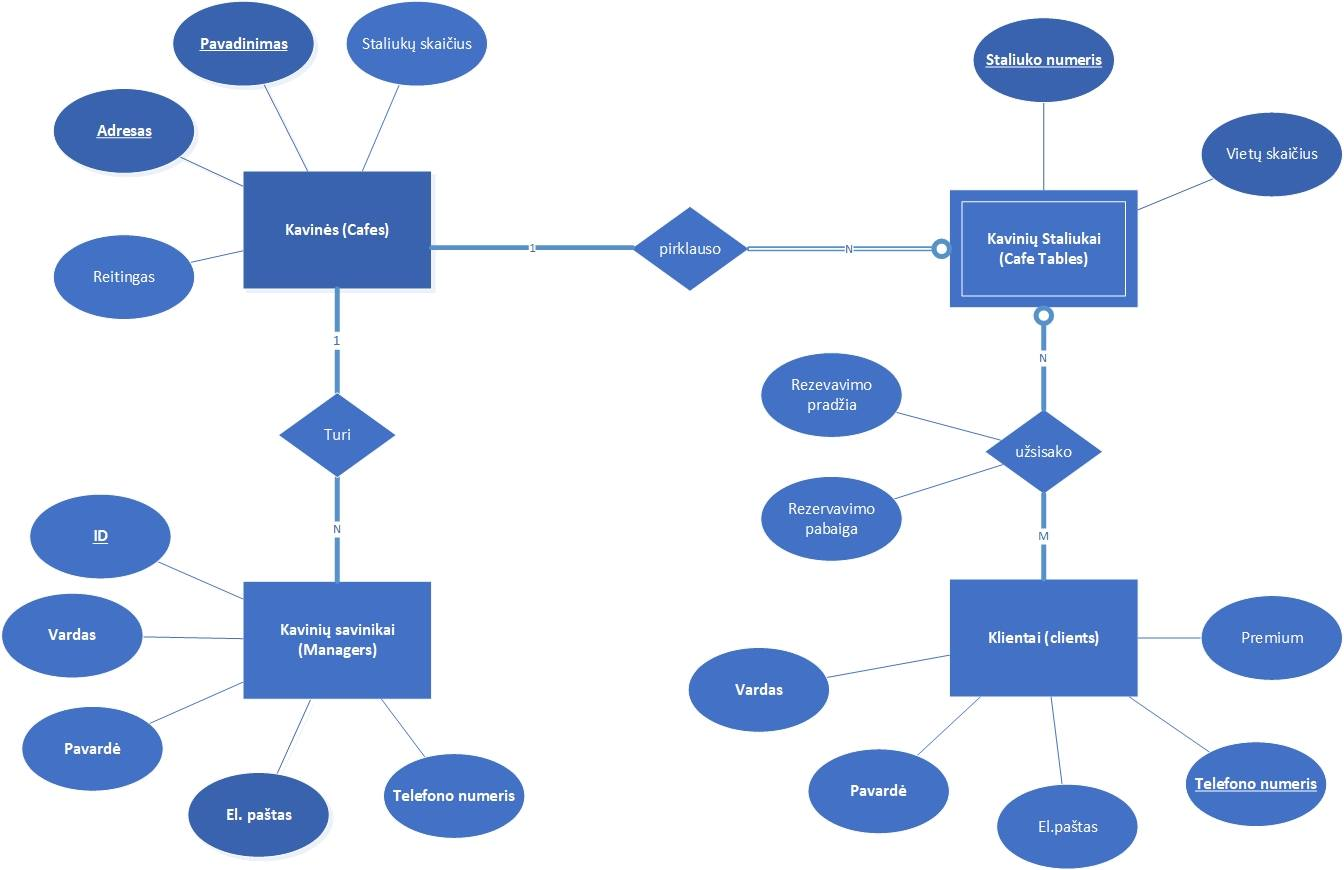
\includegraphics[width=1.3\textwidth,height=1.4\textheight,keepaspectratio]{img/ER}
		\caption{Duomenų bazės E-R diagrama}
		\label{fig:ER}
	\end{figure}
	
	\begin {figure}
		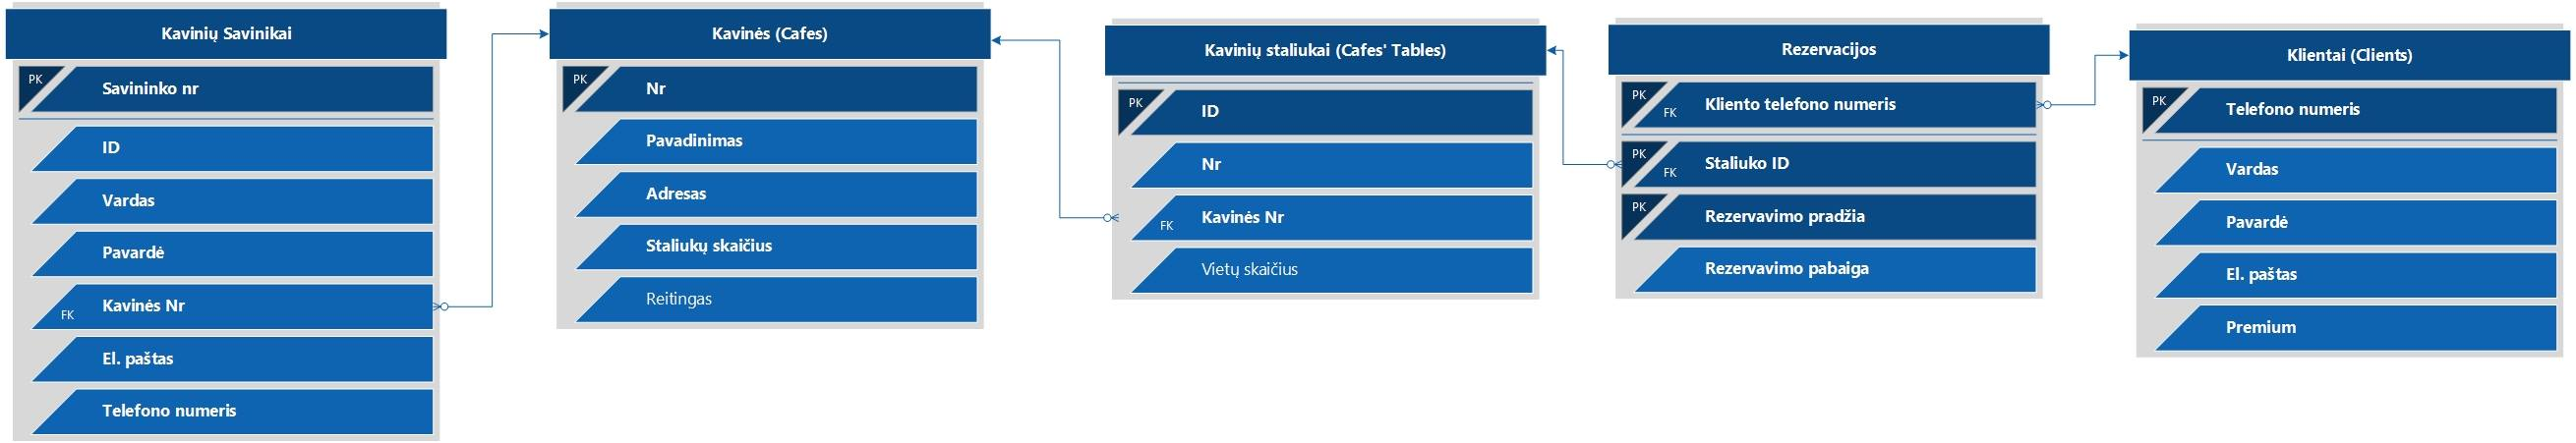
\includegraphics[width=1.5\textwidth,height=1.65\textheight,keepaspectratio]{img/lenteles}
		\caption{Duomenų bazės lentelės}
		\label{fig:lenteles}
	\end{figure}
\end{landscape}

\end{document}
